
\section{Interaction of Network Functions}
The network functions in the data plane - RAN, UPF and DNN are defined in section \ref{sec:5GDataPlane}.
\begin{figure}[htbp]
	\centering
       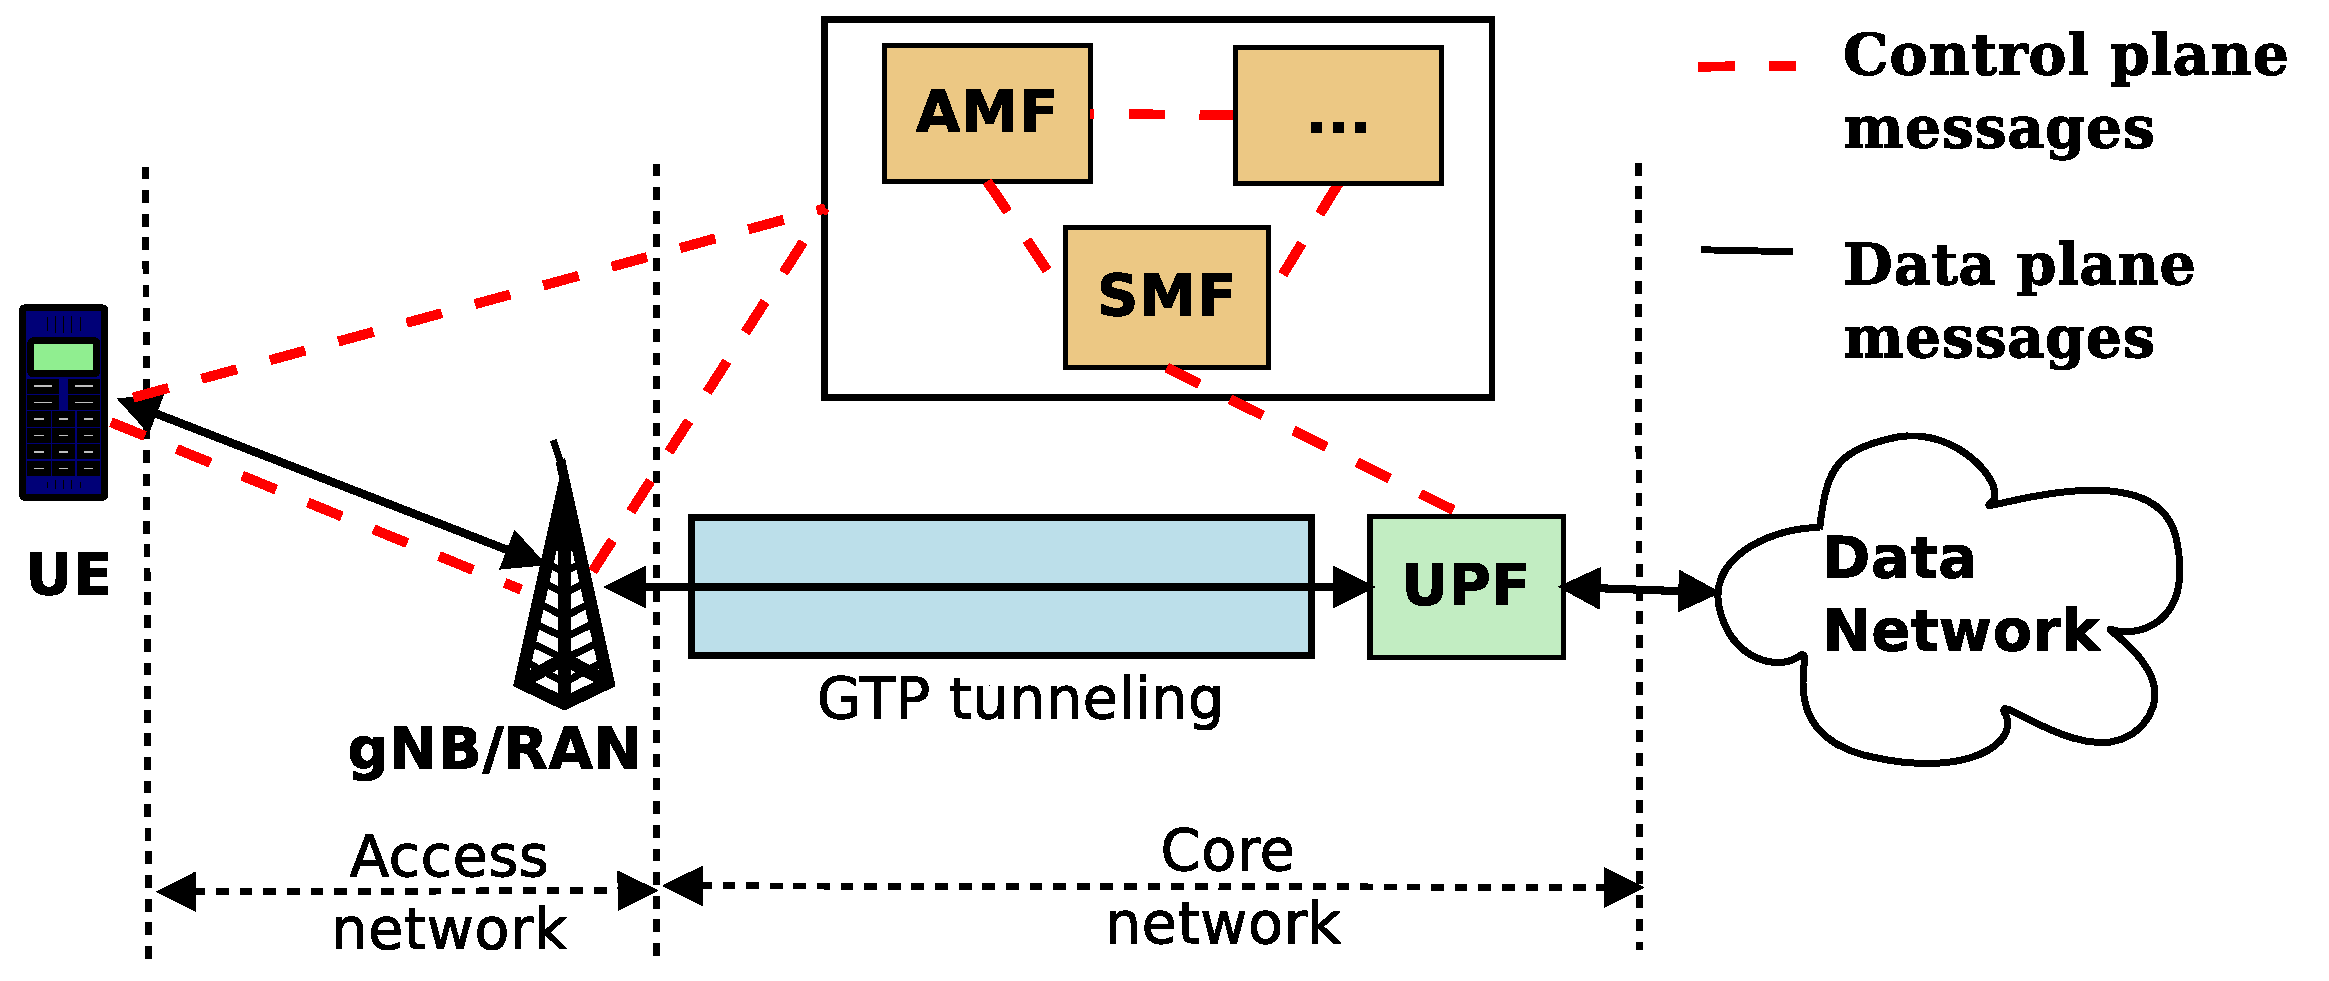
\includegraphics[width=0.7\textwidth]{fig/5g_arch.eps}
       %  \setlength{\abovecaptionskip}{-2pt}
       \setlength{\belowcaptionskip}{-12pt}
	\caption{5G Architecture.}
	\label{fig:5g_arch}
       \end{figure}
Following steps describe the interaction between various network functions during a session-
\begin{enumerate}
	\item UE interacts with the Access and Mobility function (AMF) to request for intitiation of a new session.
	\item AMF authenticates the UE and forwards the request to Session Management Function (SMF).
	\item On receiving the request from AMF and after getting the UE details from other NFs (UDR etc.),
	SMF initiates an session establishment procedure to User Plane Function. PFCP protocol (section \ref{sec:PFCP}) is used for the interaction between 
	UPF and SMF.
	\item Once the session related details are received and stored at the UPF, a confirmation is sent to the 
	UE signalling the permission to forward data packets. 
	\item Data packets are sent by the UE through RAN to the UPF. 
	\item GTP-U (section \ref{sec:GTP}) - a tunneling based protocol is used between RAN and UPF. GTP header has an identifier to map data plane packets 
	to a particular session. 
	\item UPF de-encapsulates the GTP packet and based on the stored session 
	related information provides various services like QoS, forwarding to a DNN etc. 
	\item The downlink packets are received by the UPF from the data newtork (DNN) and performs GTP encapsulation before forwarding them to the RAN/UE.  	
	\item Once the required data is forwarded, UE sends session termination request to AMF which forwards it to the SMF. SMF sends session release request to the UPF. The UPF deletes the session related information  at itself. 
\end{enumerate}
 
       %\vspace{-5mm}
       




\section {PFCP Protocol\label{sec:PFCP}}
 \begin{figure}[htbp]
    \centering
    \includegraphics[width=0.7\textwidth, keepaspectratio]{./fig/Introduction/PFCP.png}
    \caption{PFCP Session Messages}
    \label{fig:PFCP}
\end{figure}

PFCP stands for Packet Forwarding Control Protocol (\cite{5g29244}). 
 There are two types of messages sent using PFCP - node related and session related.
 The discussion here describes session related messages.

 Session Management Function (SMF) interacts with the User Plane Function (UPF) to setup sessions related 
 information at the UPF.
This  information enables UPF to identify data packets of different sessions coming from RAN 
and provide forwarding, usage report, charging, buffering, QoS related service to the sessions.
Each session is identified by a unique session ID which helps in differentiating 
among different UEs/sessions at the UPF. 

There are three kinds of messages sent from SMF to the UPF in PFCP session related messages-
\begin{itemize}
	\item \textbf{Establishment Request} This message has all the forwarding, usage report, QoS etc. related information for  a new UE session.  
	\item \textbf{Modification Request} Once the establishment response is
	received from the UPF, the UPF sends the modification request. The important field in this message is the intimation of identifier that will be used for data plane packets coming from the UPF. The data forwarding can not start before the modification response is received.
	\item \textbf{Release Request} Once the session is not required, th release 
	request is sent to the UPF signaling the tear down of the session and UPF
	 may remove this session's related information.
\end{itemize}
UPF gives response to each of the three messages. 
\section {GTP Protocol\label{sec:GTP}}
The raw packets meant for communicating outside the network are encapsulated within GTP  application level 
header. GTP (\cite{gtp_ref}) runs over UDP/IP stack. This GTP header (shown in \ref{figGTPheader})contains 
various fields for regulating the session parameters. The relevant fields are
 \begin{figure}[htbp]
    \centering
    \includegraphics[width=0.7\textwidth, keepaspectratio]{./fig/gtp.png}
    \caption{GTP-U header \cite{gtpwiki}}
    \label{figGTPheader}
\end{figure}
 \begin{itemize}
    \item \textbf{Tunnel Endpoint Identifier (TEID)} identifies the packet with a particular session which may have different Quality of Service parameters.
    \item \textbf{Extension Headers} These are required for providing differentiated services to  a given packet in the same or different session.
 \end{itemize}

